\section{\secondtitle}

\begin{frame}

\begin{block}{New formulation}

\begin{tabular}{p{15mm}p{110mm}}
  $a_{ijtt'}$ & : =1 if aircraft $i$ starts an assignment to mission $j$ at the beginning of period $t$ and finishes at the end of period $t'$, zero otherwise.  \\
  $m_{ip}$ &: =1 if aircraft $i$ uses check pattern $p$, zero otherwise.
 each pattern $p$ has a single feasible combination of check starts for an aircraft during the whole planning (usually only 1-2 checks per aircraft). \\
\end{tabular}

\begin{align}
  & \sum_{(j, t, t') \in \mathcal{J}\mathcal{T}\mathcal{T}_{ic}} a_{ijtt'} H^\prime_{jtt'} + U^{\prime}_{tc} \leq H^{M} + M (1 - m_{ip}) & \notag \\
  & \hspace{200px}  i \in \mathcal{I}, p \in \mathcal{P}, c \in \mathcal{C}_p \label{eq:cycle_hours2}\\
\end{align}

\end{block}

\end{frame}

\begin{frame}

\begin{block}{Formulation}

\begin{align}
  & \text{Max}\;
  \sum_{i \in \mathcal{I}, p \in \mathcal{P}} m_{ip} \times W_p \\
  & \sum_{i \in \mathcal{I}, p \in \mathcal{P}_{t}} m_{ip} \leq C^{max} 
          & t \in \mathcal{T} \label{eq:capacity1}\\
  & \sum_{i \in \mathcal{I}_j, (t_1, t_2) \in \mathcal{T}_{jt}} a_{ijt_1t_2} \geq R_j
          & j \in \mathcal{J}, t \in \mathcal{TJ}_j  \label{eq:missionres}\\
  & \sum_{p \in \mathcal{P}_{t}} m_{ip} + \sum_{j \in \mathcal{J}_t \cap \mathcal{J}_i} \sum_{(t_1, t_2) \in \mathcal{T}_{jt}} a_{ijt_1t_2} \leq 1 
          & t \in \mathcal{T}, i \in \mathcal{I} \label{eq:state}\\
  & \sum_{(j, t, t') \in \mathcal{J}\mathcal{T}\mathcal{T}_{ic}} a_{ijtt'} H^\prime_{jtt'} + U^{\prime}_{tc} \leq H^M + M (1 - m_{ip}) & \notag \\
    & & i \in \mathcal{I}, p \in \mathcal{P}, c \in \mathcal{C}_p \\
\end{align}

\end{block}

\end{frame}

\begin{frame}

\begin{block}{New vs old formulation}

\begin{enumerate}[<+->]

\item
  It uses 3 times the number of constraints and 3 times the number of
  variables.
\end{enumerate}

\begin{itemize}[<+->]

\item
  variables: 11000 =\textgreater{} 28000.
\item
  constraints: 13000 =\textgreater{} 48000.
\end{itemize}

\begin{enumerate}[<+->]

\item
  It is still better. Better lineal relaxation, better performance.
\item
  Can we reduce intelligently the number of variables?
\end{enumerate}

\begin{itemize}[<+->]

\item
  we can.
\end{itemize}

\end{block}

\end{frame}

\begin{frame}

\begin{block}{Predicting pseudo-cuts}

Let an optimization problem with input data \(x\) and solution space
\(y \in \mathcal{Y}(x)\). We want to find the optimal solution given a
cost function \(C(x,y)\):

\[
y^{*}(x) :\equiv arg \,\,\min_{y \in \mathcal{Y}(x)} C(x,y)
\]

For any solution \(y\), we can calculate \(N\) several features
\(g_n(y) \,\, \forall n \in \{1, .., N\}\).

\[
\hat{g}_n(x) \approx g_n(y^{*}) \,\, \forall n \in \{1, .., N\}
\]

We then use that information to reduce the solution space
\(\mathcal{Y}^\prime(x) \subset \mathcal{Y}(x)\) and solve it:

\[\hat{y}^{*}(x) = arg \,\,\min_{y \in \mathcal{Y}^\prime(x)} C(x,y)\]

The trick is doing so without losing optimality:

\begin{align}
    C(x,\hat{y}^{*}(x)) \approx  C(x,y^{*}(x) ) \notag
\end{align}

\end{block}

\end{frame}

\begin{frame}

\begin{block}{Distance between maintenances}

.pull-left{[} * The distance between maintenance has a maximum of
\(E^{M}\) periods. * Depending on the instance, the optimal distance can
be shorter. * This distance conditions the total number of patterns to
create.{]}

.pull-right{[}

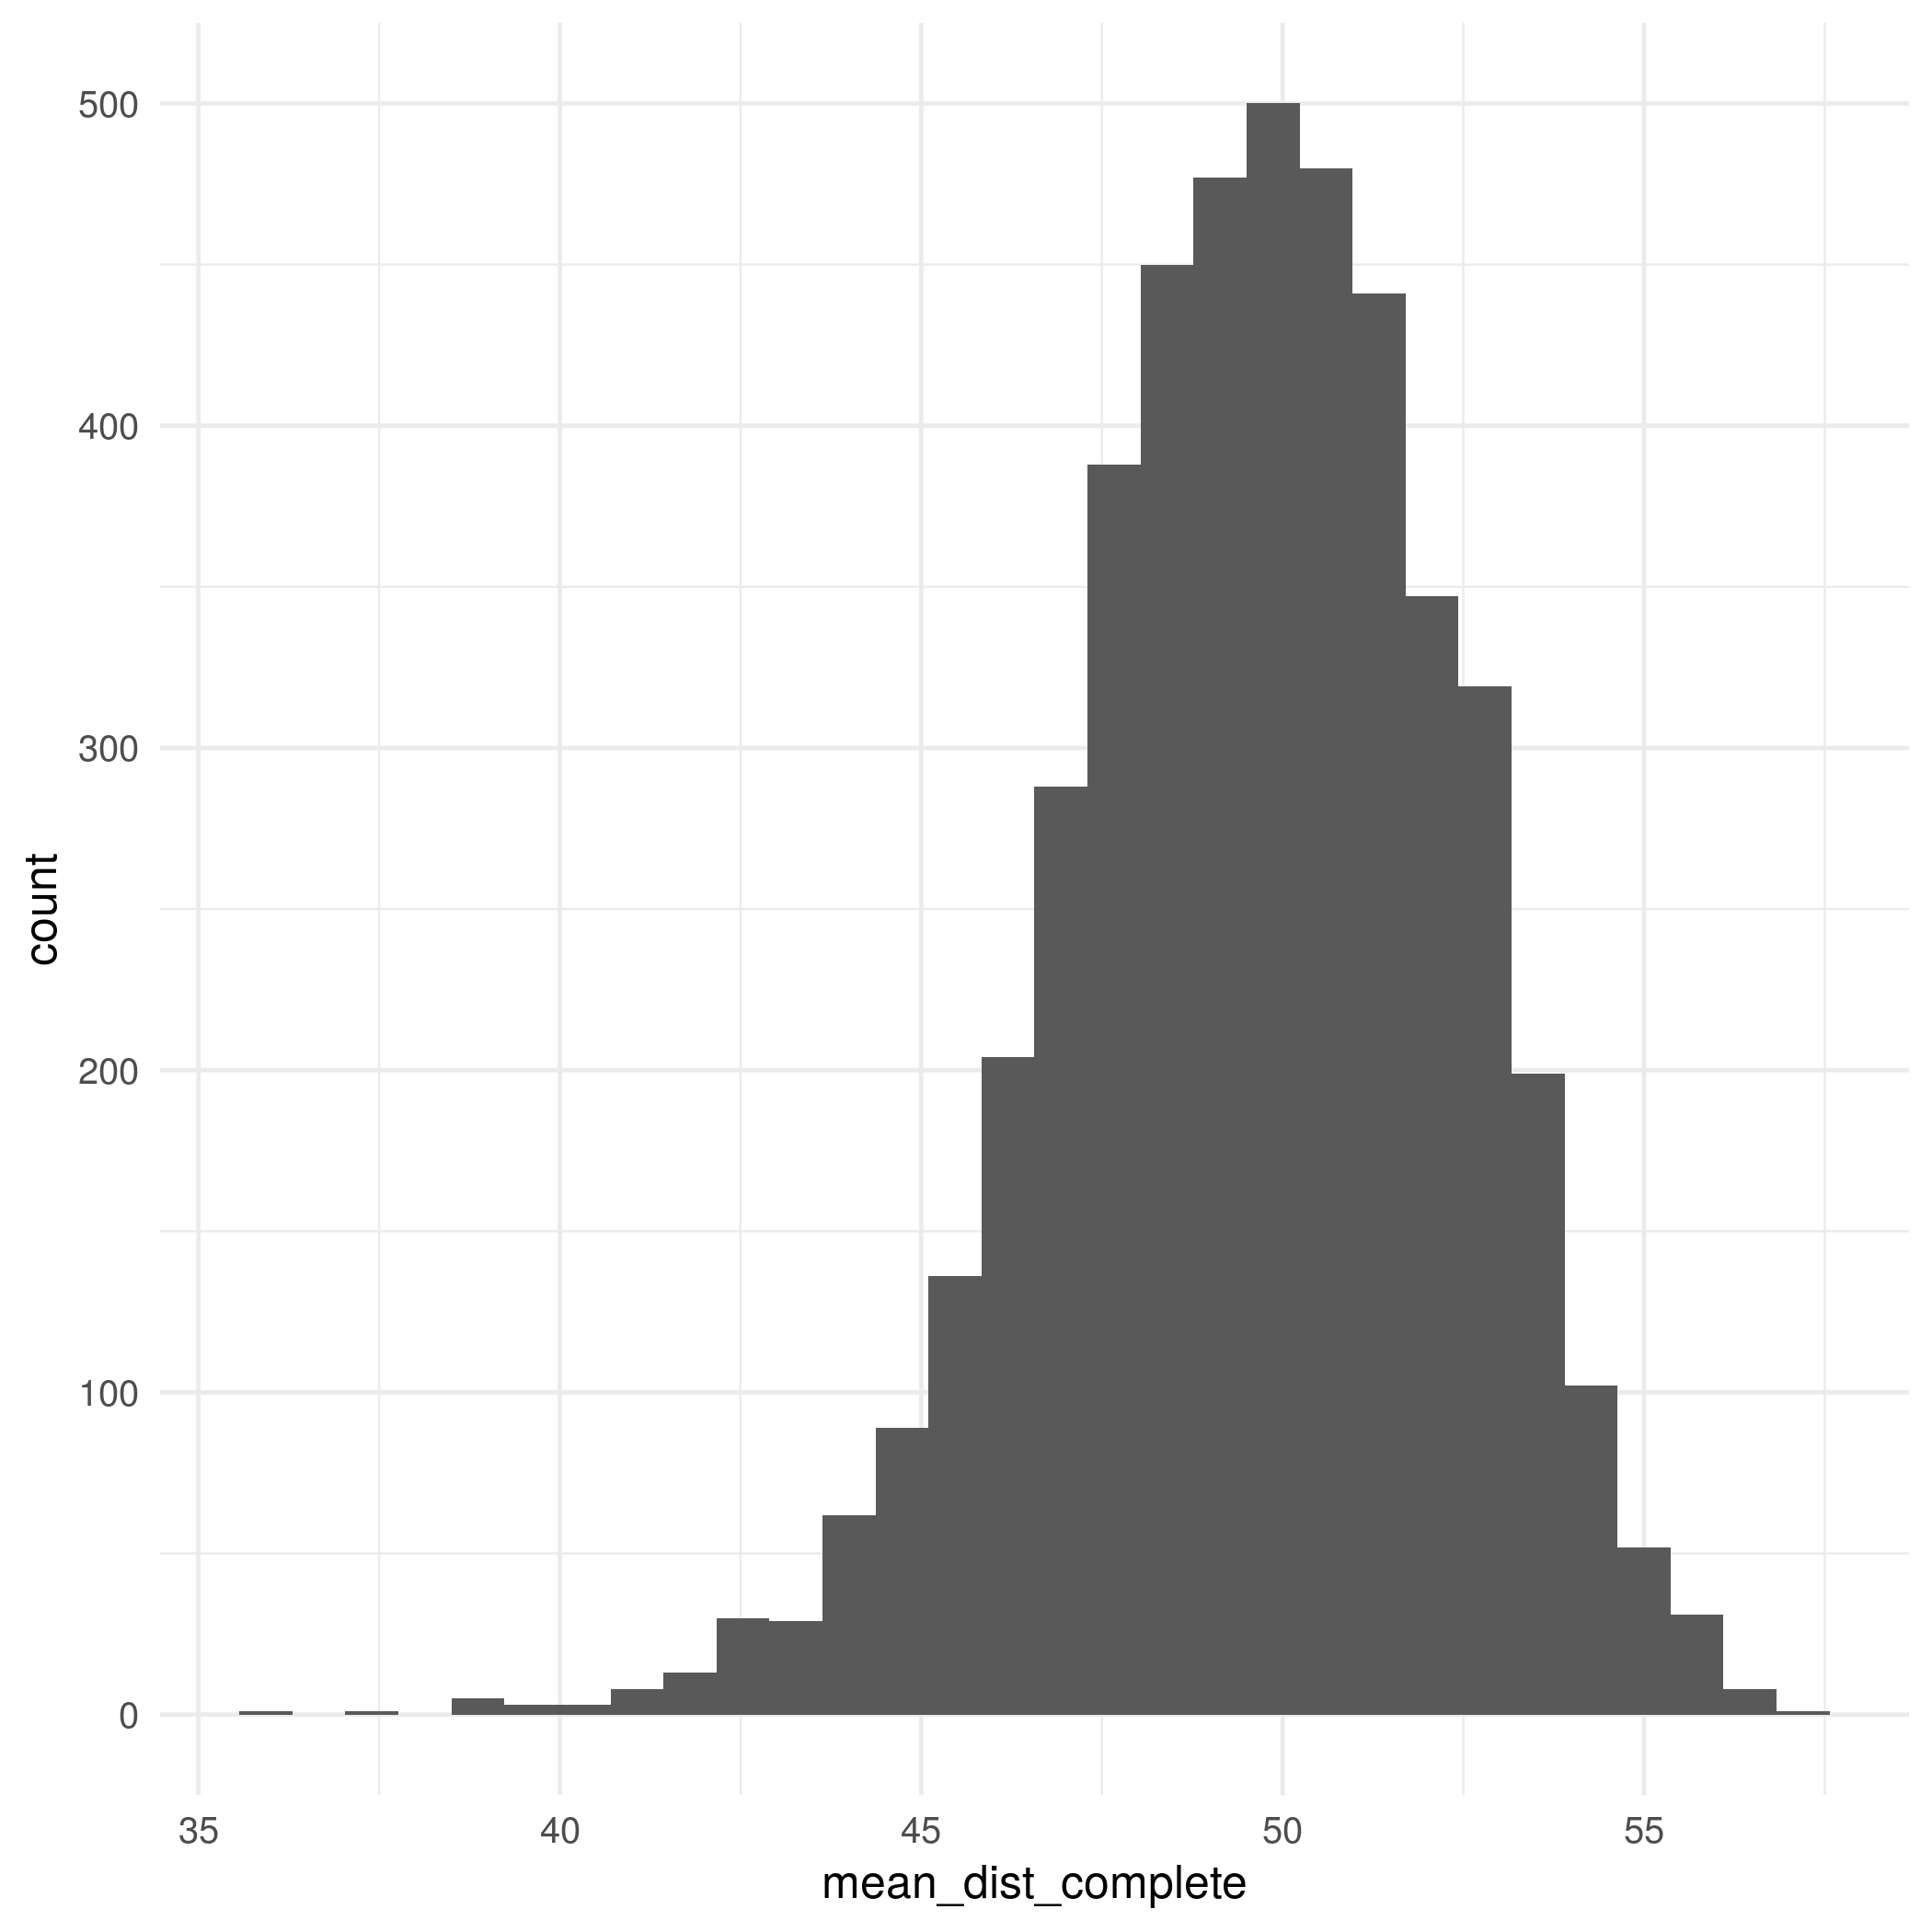
\includegraphics[width=1\linewidth]{hist_mean_dist_complete_IT000125_20190716}
{]}

\end{block}

\end{frame}

\begin{frame}

\begin{block}{Forecasting + Optimization}

\textbf{We want to}:

\begin{enumerate}[<+->]

\item
  Train a statistical model to predict the mean distance between
  maintenances for any given instance.
\item
  Use this information to limit all possible combinations of patterns to
  generate.
\end{enumerate}

--

\textbf{Benefits}:

\begin{enumerate}[<+->]

\item
  \textbf{Performance}: a smaller model is easier to solve.
\item
  \textbf{User feedback}: direct feedback about the solution without
  needing to solve any model.
\item
  \textbf{More stable solutions}: Every aircraft flies an amount that is
  closest to the mean of the fleet.
\end{enumerate}

--

\textbf{The better we're able to predict the optimal distance between
maintenances for the whole fleet, the less optimality we will lose}

\end{block}

\end{frame}

\begin{frame}

\begin{block}{Prediction model}

.pull-left{[} * \textbf{Technique}: \emph{Quantile regressions} to
estimate upper and lower bounds. * \textbf{Training}: 5000 small
instances. * \textbf{Input features}: * mean flight demand per period, *
total remaining flight hours at start (init), * variance of flight
demand, * demand of special missions, * number of period where flight
demand is cut in two. * \textbf{Output features}: mean distance between
maintenances.{]}

--

.pull-right{[}

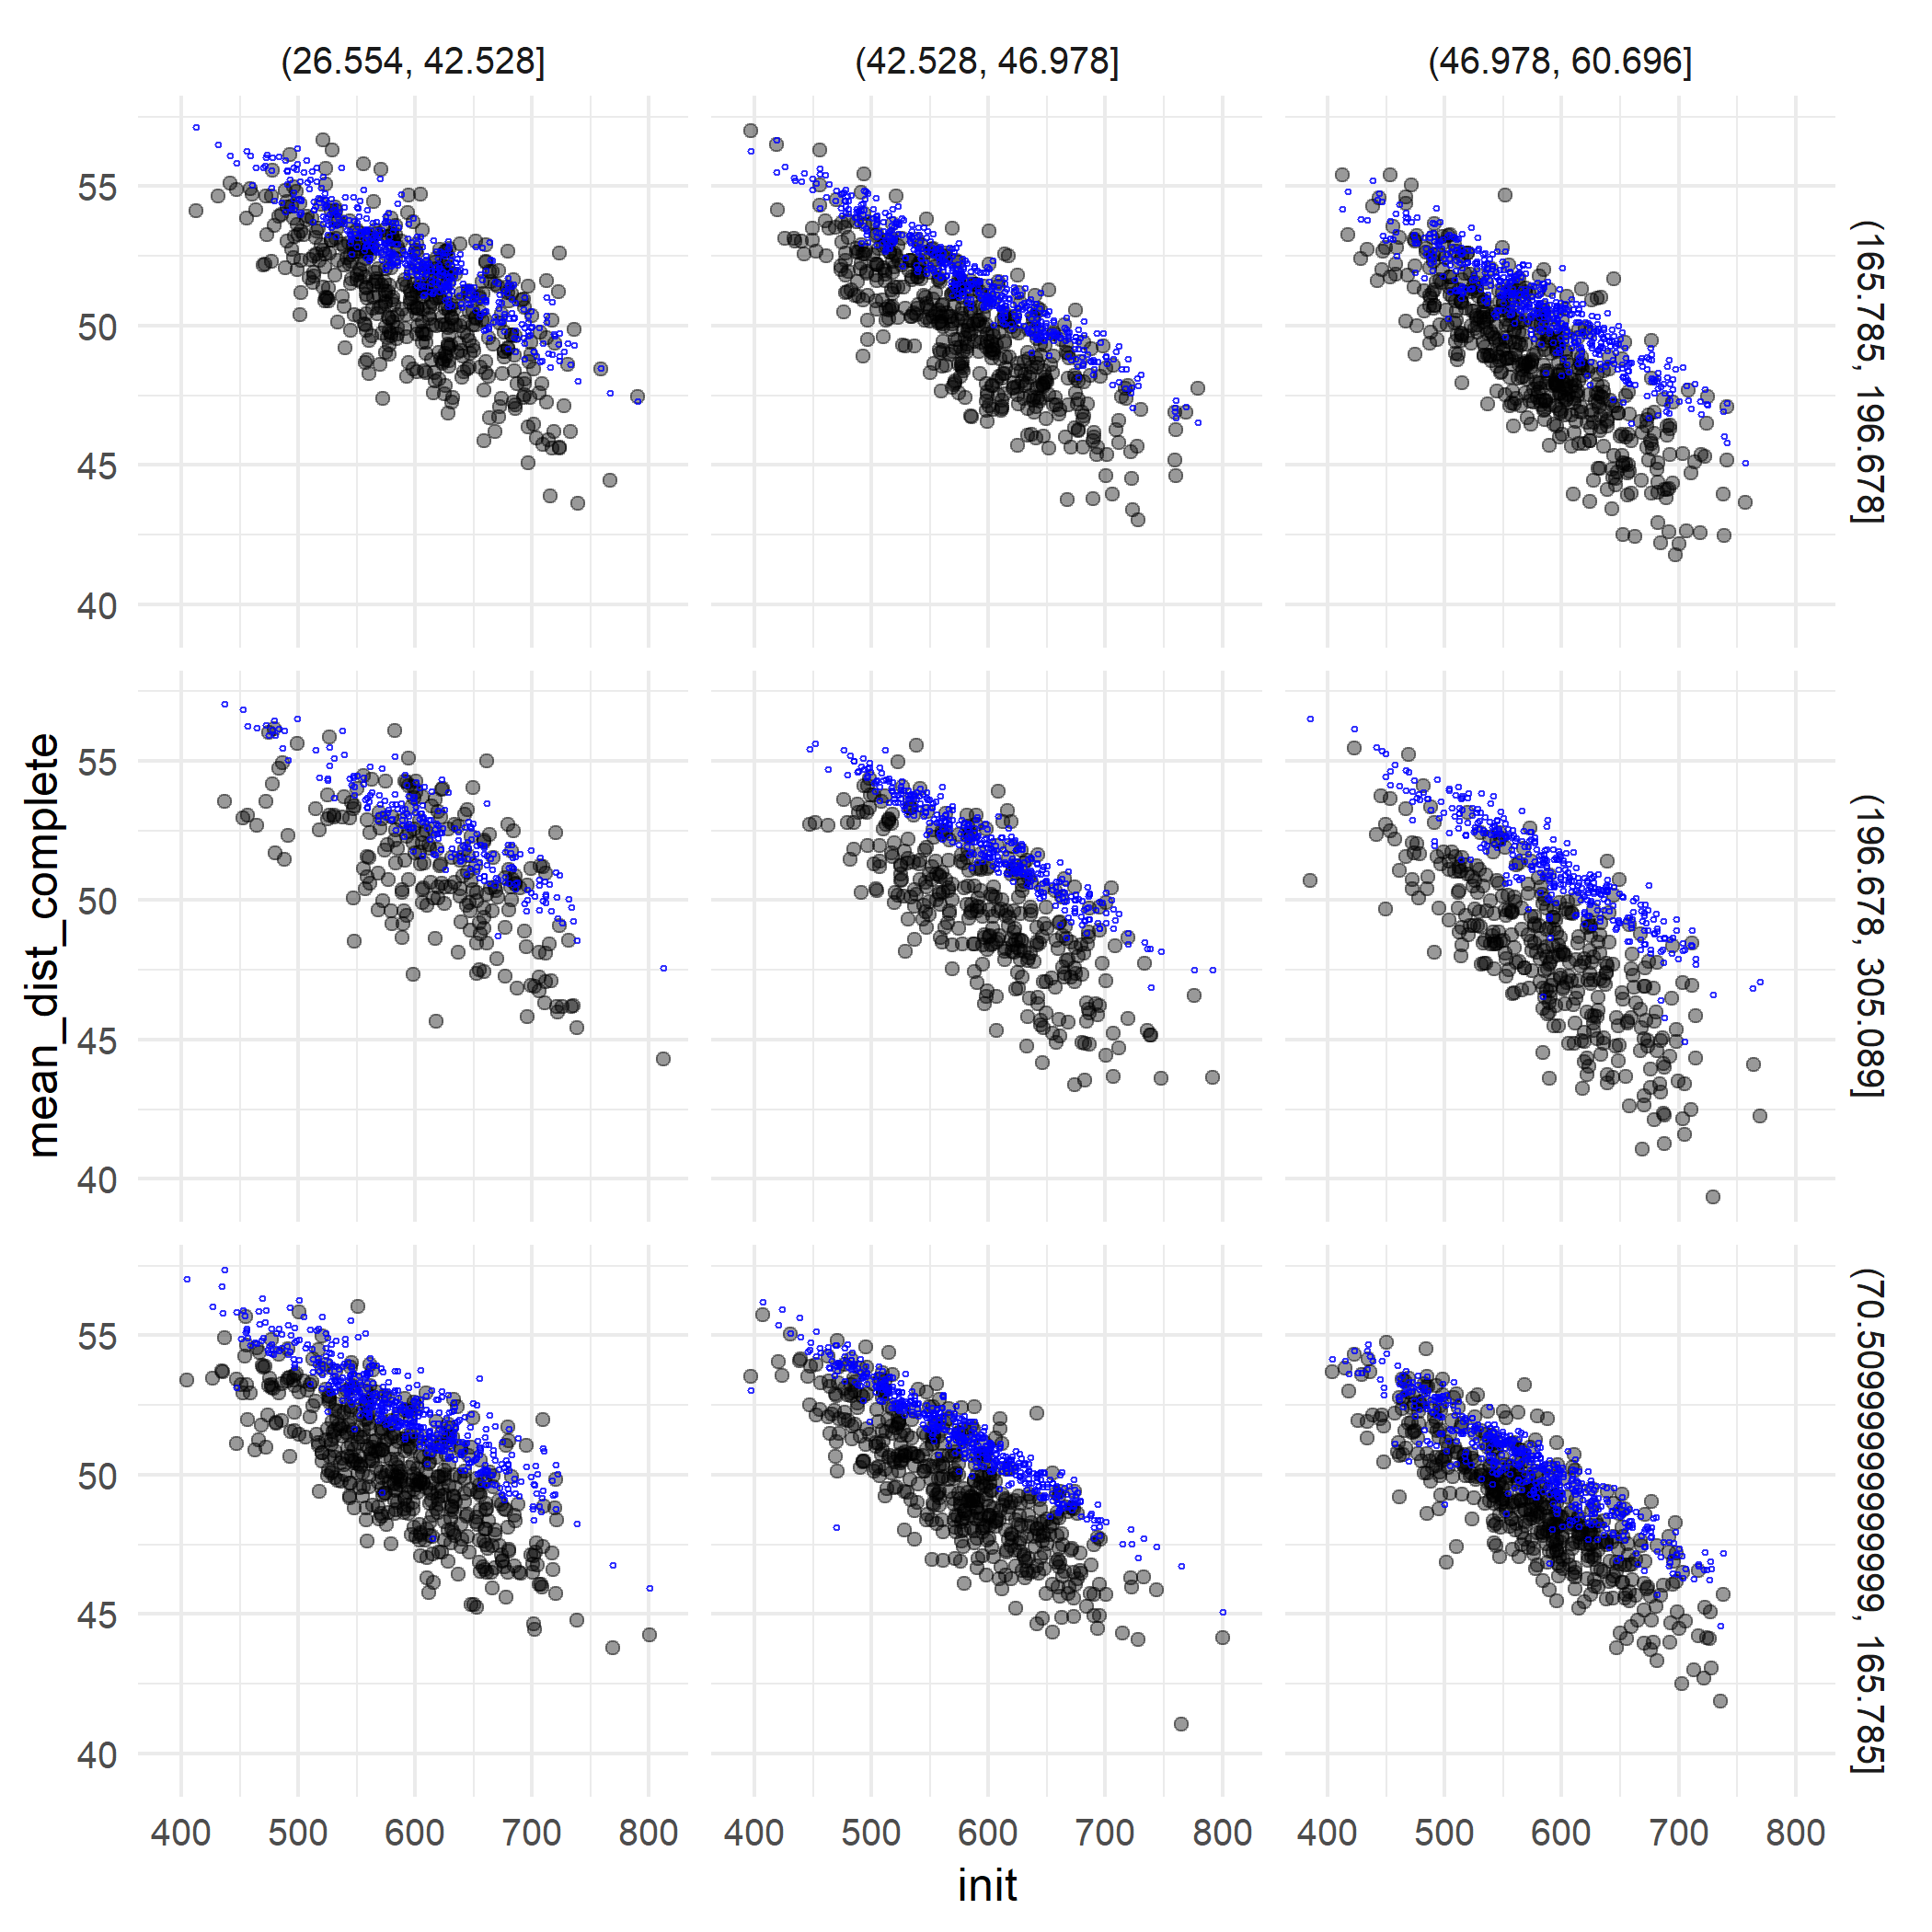
\includegraphics[width=1\linewidth]{QuantReg_mean_consum_upper_mean_dist_complete_IT000125_20190716}
{]}

\end{block}

\end{frame}

\begin{frame}

\begin{block}{Experiments}

\begin{itemize}[<+->]

\item
  Number of instances: medium (1000), large (1000) and very large
  (1000).
\item
  Time limit at 3600 seconds.
\item
  We seeded instance generation for better comparison.
\item
  CPLEX running 1 thread.
\end{itemize}

--

Largest instances have 60 aircraft, 90 periods, \textasciitilde{}30
missions (4 active missions at any given time).

\begin{enumerate}[<+->]

\item
  Create forecasting model based in 5000 small instances.
\item
  Use forecasting model to predict bounds on distance between
  maintenances: \(\hat{\mu}_{t'-t}^{lb}\), \(\hat{\mu}_{t'-t}^{ub}\).
\item
  Implement the pseudo-cut:
\end{enumerate}

\begin{align}
    & m_{ip} = 0 & p_{t'} - p_t < \hat{\mu}_{t'-t}^{lb} - tol \label{eq:dist_lb} \\
    & m_{ip} = 0  &  p_{t'} - p_t > \hat{\mu}_{t'-t}^{ub} + tol \label{eq:dist_ub}
\end{align}

\begin{enumerate}[<+->]
\setcounter{enumi}{3}

\item
  Recycling.
\end{enumerate}

\end{block}

\end{frame}

\begin{frame}

\begin{block}{How good is it (performance)}

Faster solutions, more solutions.

--

.center{[}

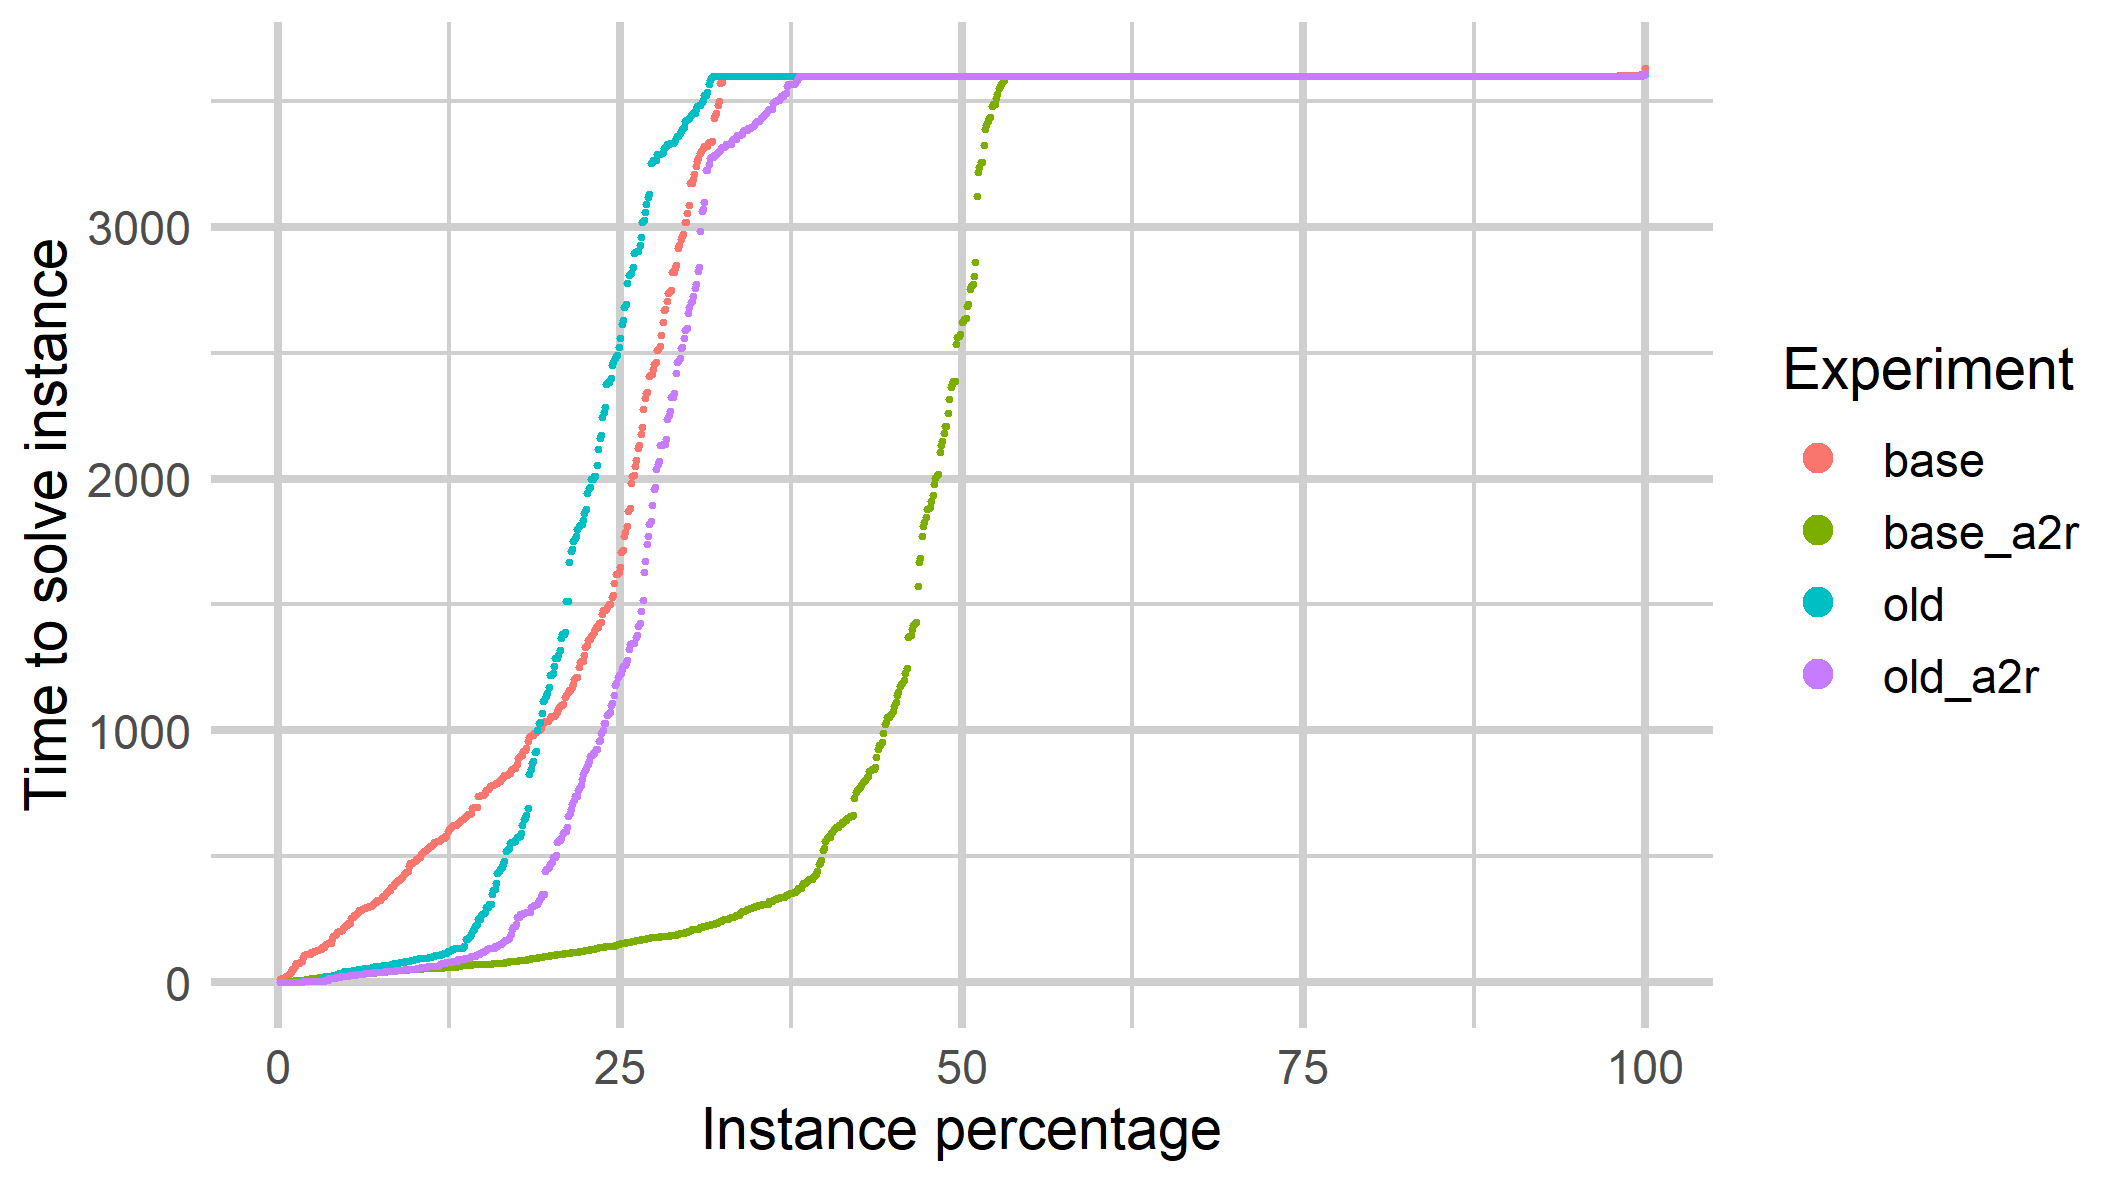
\includegraphics[width=0.8\linewidth]{time_performance_ordered_2tasks}
{]}

\end{block}

\end{frame}

\begin{frame}

\begin{block}{How good is it (optimality)}

For instances were an optimal solution was found (optimum degradation):
* 95\% of instances had less than 4\% gap with real optimal.

.center{[}

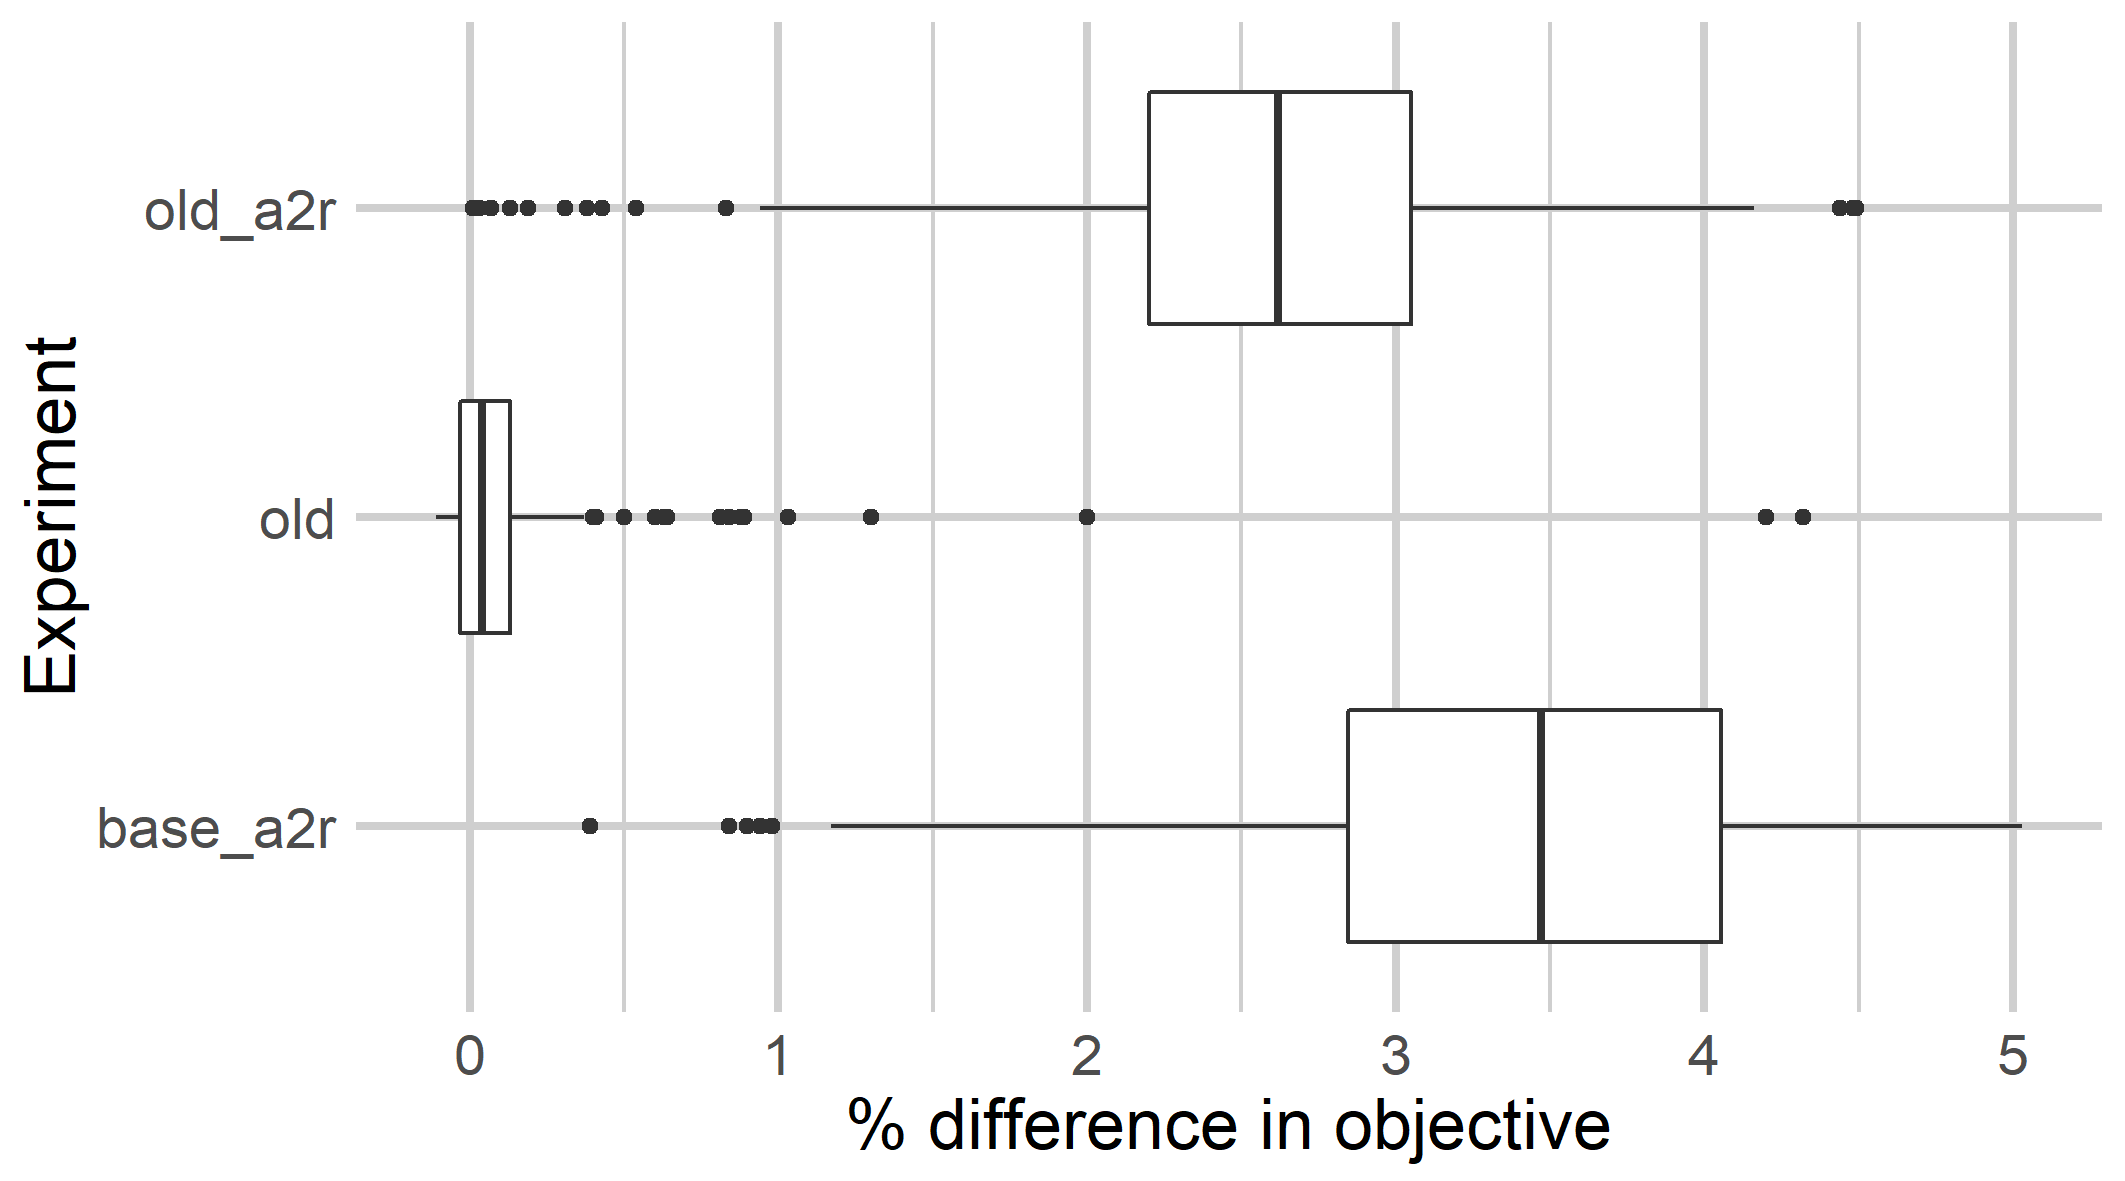
\includegraphics[width=0.8\linewidth]{quality_degradation_2tasks} {]}

\end{block}

\end{frame}

\begin{frame}{Further steps}
\protect\hypertarget{further-steps}{}

\begin{itemize}[<+->]

\item
  \textbf{Better predictions} with better features, or predicting
  several characteristics of optimal solutions.
\item
  \textbf{Predict a distribution} and sample patterns from the
  distribution instead of predicting patterns.
\item
  \textbf{Warm-start Column Generation} with a selected subset of
  potentially good patterns.
\item
  \textbf{Automatize prediction} so it can be easily integrated in other
  problems.
\end{itemize}

\end{frame}